% !TeX spellcheck = en_US
\RequirePackage{ifluatex, ifxetex} % these are for the portability of this example - can be omitted in any actual document made for a certain engine

\ifnum 0\ifxetex 1\fi\ifluatex 1\fi>0
\else
  % only needed for using Greek letters outside math when running PDFLaTeX - leave out otherwise
  %\PassOptionsToPackage{LGR}{fontenc}
  %\RequirePackage{textgreek}
\fi

% Own environment definitions.
\newenvironment{it} {\itshape}


\documentclass[globalnumbering,centeredcaptions,draftfooter]{tutthesis} % see appendix for list of options

\pagestyle{headings} % Adds titles to the header


% ifnameyear is defined to demonstrate both versions in a single file. You may leave it out and simply use one version throughout your file.
\newif\ifnameyear
\nameyearfalse



% ==============
% Basic packages
% ==============
% You should use these unless you really know what you're doing

\ifnum 0\ifxetex 1\fi\ifluatex 1\fi>0
\else\usepackage[utf8]{inputenc}
\fi

\usepackage[english,finnish]{babel} % The language of the thesis last

% If you are working with a minimal LateX distribution, you may have to install some extra packages. Make sure that at least babel-finnish (available in e.g. texlive-lang-european) and the basic fonts (e.g. texlive-fonts-recommended) are installed.

\usepackage{babelbib} % You should use this unless you are using biblatex. Add option fixlanguage if you're writing in English (the thesis writing guide is asymmetric, requiring Finnish theses to have e.g. 'eds.' for sources in English, while requiring English theses to have all such parts in English)

\ifnameyear\usepackage{natbib} % add option longnamesfirst if you want to have full author list with first citation
\else\providecommand{\citep}{\cite} % This template is written using \citep to get name-year citations right, and in numerical mode the command is here aliased to the standard \cite. If you use numbered citations, leave this out and use \cite
\fi

% Path to search graphics used in this document.
\graphicspath{pictures/}


% ===============
% Useful packages
% ===============
% Packages which are not required for a thesis that follows guidelines, but may be convenient or necessary in common cases

%\usepackage{microtype} % subtle but nice improvements to how text is printed

%\usepackage{textcase} % may be used to keep parts of title lowercase
\usepackage{array}
\usepackage{tabularx} % e.g. multiline cells
%\usepackage{calc} % for performing length arithmetic such as column width = text width minus some other width
%\usepackage{longtable} % for tables spanning multiple pages

%\usepackage{psfrag} % editing ps files
%\usepackage{subfig} % parallel small figures a,b,c,...
%\usepackage{rotating} % for rotating e.g. full-page figures

%\usepackage{siunitx} % nice formatting for combinations of number and unit
\usepackage{amsopn} % For operator names; not necessary if amsmath is used
%\usepackage[fleqn]{amsmath} %Extensions to math handling; if you use this, you should use e.g. gather instead of equation due to a hyperref bug

\usepackage{listings} %Typesetting code
%\lstset{basicstyle=\footnotesize\ttfamily, numbers=left}
\renewcommand{\lstlistingname}{Ohjelma} % Rename "Listing" to "Ohjelma".
% If you want non-ASCII characters (e.g. in comments), check out the listingsutf8 package

\ifnum 0\ifxetex 1\fi\ifluatex 1\fi>0
  \usepackage[math-style=ISO]{unicode-math} %must not precede amsmath and most other math and font related packages
\else
  %\usepackage{bm} % The \bm command is used for bold italic variables used in some fields not to be used with unicode-math
  %\usepackage[helvratio=1]{newtxtext} \usepackage{newtxmath}% some recommend the newtx fonts
  \usepackage{textcomp} % symbols like \textdegree
\fi


% ===========================
% Bibliographic information
% ===========================
% These must be set before loading pdfx or beginning document
\author{Mauri Mustonen}
\title{sähköaseman älykkään elektroniikkalaitteen viestien tilaus ja prosessointi}
\datesubmitted{2018}{5}{17} % year, month, day; no leading zeroes; submitted for bachelor's theses and thesisapproved for master’s
\thesistype{Diplomityö} % Do not use ASCII apostrophe ' as it will not be substituted with the correct one (’) in the PDF metadata. Note that there are both short version (this) and a long one - "Master’s" vs. "Master of Science"
\major{Ohjelmistotuotanto}
\programme{Tietotekniikan koulutusohjelma} % Note apostrophes on all fields for PDF metadata
\examiner{Prof. Kari Systä} %\and for plural
%\datetopicapproved{2017}{1}{5} % only for master’s theses
\keywords{IEC 61850, MMS, AMQP}


% Packages that need to be loaded late
% ----------------------------------------------
% \usepackage[a-2u]{pdfx} % If you're using PDFLatex and your version of pdfx is not recent enough, you may run into the inputencoding bug. In that case, load inputenc after pdfx (and replace any non-ASCII characters in the metadata with e.g. \"{a})

\usepackage{hyperref} % This must (usually) be the last package you load - load this OR pdfx (which also loads hyperref). Usage of pdfx would be nice, but if you have issues with that you may fall back to just hyperref



\begin{document}


\maketitle
%First, the abstract in the language of the thesis (no language selection). Note that most fields are already defined.
\thesisdescription{Diplomityö}


\begin{abstract}
% TODO: Muokkaa tätä vastaamaan uutta kirjoitusta mikäli tarve vaatii.
Sähkönjakeluverkko on tärkeä osa nykyistä yhteiskuntaa ja sen päivittäistä toimintaa. Sähköverkko koostuu sähköntuotantolaitoksista, sähkölinjoista ja sähköasemista. Sähköverkon eri komponenttien avulla sähkö toimitetaan tuontantolaitoksesta kuluttajille. Sähköasemat ja niiden automatisointi ovat tärkeässä roolissa verkon yleisen toiminnan ja turvallisuuden takaamiseksi. Tässä diplomityössä keskitytään suunnittelemaan ja toteuttamaan yksittäinen ohjelmistokomponentti osaksi isompaa sähköasemiin liittyvää järjestelmää. Suunniteltavan komponentin tarkoituksena on tilata tietoa sähköasemalta verkon yli ja saada jaettua tämä tieto järjestelmän muille komponenteille. Sähköasemalta tuleva tieto on esimerkiksi mittaustietoa ja mittaustiedosta kiinnostunut järjestelmän komponentti tarvitsee tämän tiedon käyttöliittymässä näyttämiseen.

Sähköasemilta tieto tilataan \emph{älykkäiltä elektroniikkalaitteilta} (engl. \emph{Intelligent Electronic Device}, \emph{IED}). IED:t ovat sähköaseman automaatiolaitteita, jotka on kytketty aseman verkkoon. Näistä käytetään myös nimitystä suojarele. IED-laitteiden kommunikointiin liittyy vahvasti maailmanlaajuinen \emph{IEC 61850} -standardi (engl. \emph{International Electrotechnical Commission}). Standardi määrittää kuinka IED-laitteet kommunikoivat verkon yli ja mekanismit kuinka ulkopuolinen ohjelma voi tilata siltä viestejä.

Ennen työn aloitusta ohjelmasta oli toteutettu demo, joka todisti kokonaisuuden toimivuuden. Demototeutuksessa oli kuitenkin ongelmia, jotka estivät sen käytön luotettavasti tuotannossa. Tässä työssä demoa käytettiin pohjana uuden version suunnittelulle. Demosta analysoitiin sen ongelmia ja mistä ne johtuivat. Näitä tietoja käytettiin uuden komponentin suunnitteluun liittyvissä päätöksissä.

Tuloksena työstä oli muusta järjetelmästä riippumaton ohjelmistokomponentti, joka pystyi tilaamaan viesteja IED-laitteelta IEC 61850 -standardin mukaisesti. Komponentti kykeni prosessoimaan ja jakamaan tilatut viestit järjestelmän muiden komponenttien kanssa. Komponentti päätyi tuotantoon osaksi muuta järjestelmää.
\end{abstract}


%Then, the abstract in the other language (explicit language selection) except for bachelor's theses
\begin{otherlanguage}{english}

\title{Substation’s intelligent electronic device messages subscription and processing}
\programme{Master’s Degree Programme in Information Technology}
\thesisdescription{Master of Science thesis}
\major{Software Engineering}
\examiner{Prof. Kari Systä}
\keywords{IEC 61850, MMS, AMQP}

\begin{abstract}
Nowadays an electric grid is an important part of our society. It consists of power plants, power lines and substations. With these components' electricity can be delivered from power plants to the end users. Substations and their automation play an important role in guaranteeing power grid safety and functionality. The focus of this master thesis is to plan and implement distributed system architecture and a software component. Both to be a part of the bigger system which is related to substations and their management. The implementation should be able to subscribe information from the substation and share it with other parts of the system. The information from the substation can include different types of data such as measurement data which for example can be shown on the user interface.

The information is subscribed in substations from an Intelligent Electronic Device, IED for short. An IED is an automation device which controls the other physical devices of the substation. IEDs are also connected to the substation's local network. IED can also be called with the name protection relay. The International Electrotechnical Commission has defined a worldwide standard called IEC 61850 which defines the rules how IED devices should communicate with each other over the substation network. This standard also defines rules for how a software outside the substation network need to communicate with them.

Distributed system architecture is planned by analyzing different communication paradigms and selecting ones that seem to solve the problem best. Before this thesis started, a proof of concept software component had already been developed. However, this component had many problems which did not encourage its development further. Analyzing these problems is a part of this thesis. The new knowledge will help to plan new software's technical side.

As a result, from this thesis is a distributed system architecture and a software component. Implementation can subscribe information from the IED according to the IEC 61850 standard and share it with the other parts of the system.
\end{abstract}
\end{otherlanguage}


\chapter*{Alkusanat}
\label{ch:alkusanat}

\begin{it}
	Mistä tämän diplomityönaiheen sain ja kiittää eri ihmisiä ketä työssä oli sidoshenkilöinä.
\end{it}

\vspace{2\baselineskip}

Tampereella, 19.4.2018

\vspace{2\baselineskip}

Mauri Mustonen


% Create table of content.
\tableofcontents


% List of figures and tables.
\listoffigures
\listoftables


\chapter*{Lyhenteet ja merkinnät}
\label{ch:lyhenteetjamerkinnat}
% This is not a "proper" table, so no table environment
% Suppressed left colsep; 20% - 1 x colsep; right colpsep; left colpadding; 80% - 1 x colpadding; suppressed right colpadding
\begin{tabularx}{\linewidth}[h]{@{} p{0.2\textwidth-\tabcolsep} p{0.8\textwidth-\tabcolsep} @{}}
	ACSI & engl. \emph{Abstract Communication Service Interface}, IEC 61850 -standardin käyttämä lyhenne kuvaamaan palveluiden abstraktimalleja \\
	AMQP & engl. \emph{Advanced Message Queuing Protocol} on avoin standardi viestien välitykseen eri osapuolien kesken \\
	BRCB & engl. \emph{Buffered Report Control Block} on IEC 61850 -standardissa puskuroitu viestien tilaamisesta vastaava luokka \\
	CDC & engl. \emph{Common Data Class} on IEC 61850 -standardissa joukko uudelleenkäytettäviä dataobjekin luokkia \\
	CMV & engl. \emph{Complex Measured Value} on IEC 61850 -standardissa dataobjektin luokkatyyppi \\
	DA & engl. \emph{Data Attribute} on IEC 61850 -standardissa käsite abstrahoimaan jokin sähköaseman laitteen mitattava arvo (esim. jännite) \\
	dchg & engl. \emph{data change} on IEC 61850 -standardissa oleva liipaisimen tyyppi \\
	DO & engl. \emph{Data Object} on IEC 61850 -standardissa käsite abstrahoimaan joukko samaan kuuluvia data-attribuutteja \\
	DPC & engl. \emph{Controllable Double Point} on IEC 61850 -standardissa dataobjektin luokkatyyppi nimeltään Pos \\
	DSM & engl. \emph{Distributed Shared Memory} on jaettu muisti, joka käyttäjälle näyttää kuin paikallinen fyysinen muisti \\
	dupd & engl. \emph{data update} on IEC 61850 -standardissa oleva liipaisimen tyyppi \\
	FC & engl. \emph{Functional Constraint} on IEC 61850 -standardissa käsite viitattujen data-attribuuttien rajoittamiseen \\
	FCD & engl. \emph{Functional Constrained Data} on IEC 61850 -standardissa viitteen tyyppi rajoittaamaan viitattuja data-attribuutteja hierarkiassa ensimmäisestä dataobjektista alaspäin \\
	FCDA & engl. \emph{Functional Constrained Data Attribute} on IEC 61850 -standardissa viitteen tyyppi rajoittamaan data-attribuutteja hierarkiassa muusta kuin ensimmäisestä dataobjektista alaspäin \\
	FFI & engl. \emph{Foreign Function Interface}, mekanismi, jolla ohjelma voi kutsua toisella kielellä toteutettuja funktiota \\
	GCS & engl. \emph{Group Communication System} tarkoittaa systeemiä, jossa kommunikoidaan joukolle osapuolia \\
	GI & engl. \emph{General Interrogation} on IEC 61850 -standardissa oleva liipaisimen tyyppi \\
	GIL & engl. \emph{Global Interpreter Lock}, Ruby-kielen tulkissa oleva globaali tulkkilukitus, joka rajoittaa yhden säikeen suoritukseen kerrallaan \\
	GVL & engl. \emph{Global Virtual Machine Lock} on sama kuin GIL, mutta eri nimellä \\
	HAL & engl. \emph{Hardware Abstraction Layer} on laitteistoabstraktiotaso abstraktoimaan laitteen toiminnallisuuden lähdekoodista \\
	IEC & engl. \emph{International Electrotechnical Commission}, on sähköalan kansainvälinen standardiorganisaatio \\
	IEC 61850 & maailmanlaajuinen sähköasemien IED-laitteiden kommunikoinnin määrittävä standardi \\
	IED & engl. \emph{Intelligent Electronic Device}, sähköaseman älykäs elektroniikkalaite (myös nimellä turvarele), joka toteuttaa aseman automaatiota \\
	IoT & engl. \emph{Internet of Things}, on verkko joka koostu siihen kytketyistä erilaisista laitteista \\
	IP & engl. \emph{Internet Protocol} on protokolla verkkoliikenteessä joka huolehtii pakettien perille toimittamisesta \\
	JRuby & on Ruby-kielen tulkki Ruby-koodin suoritukseen Java-virtuaalikoneella \\
	JSON & engl. \emph{JavaScript Object Notation} on JavaScript-kielessä käytetty notaatio objektista ja sen sisällöstä \\
	JVM & engl. \emph{Java Virtual Machine} on Java-kielen virtuaalikone Java-koodin suoritukseen \\
	LD & engl. \emph{Logical Device} on IEC 61850 -standardissa käsite abstrahoimaan joukko fyysisestä laitteesta joukko loogisesti yhteen kuuluvia laitteita \\
	LN & engl. \emph{Logical Node} on IEC 61850 -standardissa käsite abstrahoimaan fyysinen laite loogisen laitteen ryhmästä \\
	mag & on dataobjektin instanssin data-attribuutti nimeltään mag (engl. magnitude) \\
	MMS & engl. \emph{Manufacturing Message Specification} on maailmanlaajuinen standardi reaaliaikaiseen kommunikointiin verkon yli eri laitteiden välillä \\
	MMXU & engl. \emph{measurement} on IEC 61850 -standardissa loogisen noodin luokka mallintamaan mitattuja arvoja \\
	MQTT & engl. \emph{Message Queuing Telemetry Transport} on julkaisija-tilaaja-pohjainen avoin standardi kommunikointiin hajautetussa järjestelmässä \\
	MRI & engl. \emph{Matz’s Ruby Interpreter} on Ruby-kielen tulkki \\
	MV & engl. \emph{Measured Value} on IEC 61850 -standardissa on dataobjektin luokkatyyppi \\
	OptFlds & engl. \emph{Optional Fields} on attribuutti viestin vaihtoehtoisten kenttien määritykseen \\
	PD & engl. \emph{Physical Device} on IEC 61850 -standardissa käytetty käsite abstrahoimaan sähköaseman fyysinen laite \\
	phsA & dataobjektin instanssi nimeltään phsA (engl. phase A) ja tyyppiä CMV \\
	PhV & dataobjektin instanssi nimeltään phV (engl. phase to ground voltage) ja tyyppiä WYE \\
	Pos & dataobjektin instanssi tyyppiä DPC ja nimeltä Pos (engl. position) \\
	q & dataobjektin instanssin data-attribuutti nimeltään q (engl. quality) \\
	qchg & engl. \emph{quality change} on IEC 61850 -standardissa oleva liipaisimen tyyppi \\
	RCB & engl. \emph{Report Control Block}, raporttien konfigurointiin ja tilaukseen tarkoitettu luokkatyyppi IED-laitteelle \\
	RMI & engl. \emph{Remote Method Invocation} on oliopohjainen metodikutsu jossa metodi sijaitsee toisella koneella \\
	RoR & engl. \emph{Ruby on Rails} on kehys web-sovellusten kehittämiseen Ruby-kielellä \\
	RPC & engl. \emph{Remote Procedure Call} on etäproseduurikutsu jossa proseduuri sijaitsee toisella koneella \\
	SCSM & engl. \emph{Specific Communication Service Mapping} on IEC 61850 -standardin abstrahoitujen mallien toteuttaminen jollakin tekniikalla \\
	stVal & dataobjektin instanssin data-attribuutti nimeltään stVal (engl. status value) \\
	t & dataobjektin instanssin data-attribuutti nimeltään t (engl. timestamp) \\
	TCP/IP & engl. \emph{Transmission Control Protocol/Internet Protocol}, on joukko standardeja verkkoliikenteen määrityksiin \\
	TotW & dataobjektin instanssi tyyppiltään MV ja nimeltä TotW (engl. total active power) \\
	TrgOp & engl. \emph{Trigger Options} on IEC 61850 -standardissa käytetty lyhenne määritetyille liipaisimille \\
	UDP & engl. \emph{User Datagram Protocol} on pakettien lähettämisen protokolla Internet protokollan päällä \\
	URCB & engl. \emph{Unbuffered Report Control Block} on IEC 61850 -standardissa ei puskuroitu viestien tilaamisesta vastaava luokka \\
	WYE & engl. \emph{Phase to ground/neutral related measured values of a three-phase system} on IEC 61850 -standardissa dataobjektin luokkatyyppi \\
	XCBR & on IEC 61850 -standardissa luokka mallintamaan sähkölinjan katkaisijaa (engl. circuit breaker) \\
	XML & engl. \emph{Extensible Markup Language} on laajennettava merkintäkieli, joka on ihmis- ja koneluettava \\
	YARV & engl. \emph{Yet another Ruby VM} on Ruby-kielen toinen tulkki, jonka tarkoitus on korvata MRI-tulkki \\
\end{tabularx}


% Each chapter is it's own file and included here.
\chapter{Johdanto}
\label{ch:johdanto}

% TODO: Kirjoita tätä vastaamaan lopussa enemmän työn oikeita tavoitteita ja katso että alaotsikot menee yhteen muun tekstin kanssa.

Sähköverkko koostuu tuotantolaitoksista, sähkölinjoista ja sähköasemista. Sähköasemilla on erilaisia tehtäviä verkossa. Näitä ovat esimerkiksi jännitteen muuntaminen, verkon jakaminen ja sen toiminnan tarkkailu. Nykypäivänä asemien toiminnallisuutta voidaan seurata ja ohjata etäohjauksella verkon yli. Etäohjelma voi saada tietoa aseman toiminnasta ja sen tilasta. Sähköaseman yksi tärkeä tehtävä on suojata ja tarkkailla verkon toimivuutta, ja vikatilanteessa esimerkiksi katkaista linjasta virrat pois. Tällainen vikatilanne on esimerkiksi kaapelin poikkimeno, joka aiheuttaa vaarallisen oikosulkutilanteen.

Tässä diplomityössä on tarkoituksena suunnitella ohjemistoarkkitehtuuria ja toteuttaa ohjelmistoa osaksi isompaa sähköasemiin liittyvää järjestelmää. Tavoitteena on saada tietoa verkon yli sähköaseman automaatiolaitteelta ja jakaa saatu tieto järjestelmän muiden osien kanssa. Työssä käsitellään hajautetun järjestelmän paradigmoja ja analysoidaan mitkä niistä sopisivat tilanteeseen parhaiten. Analyysin tuloksien ja vaatimusten perusteella päädytään kokonaisuuden suunnitelmaan. Suunnitelma toteutetaan ohjelmistoksi, joka toimii osana olemassa olevaa isompaa järjestelmää. Toteutus jakaa sähköaseman tietoa järjestelmän muille osille, joita ovat esimerkiksi mittaustiedon näyttäminen ja aseman tilan tarkkailu.

Tieto saadaam sähköasemilla olevilta \emph{älykkäiltä eletroniikkalaitteilta} (engl. \emph{Intelligent Electronic Device}, lyhennetään \emph{IED}). IED-laite on sähköaseman automaatiolaite jota kutsutaan myös nimellä suojarele. IED-laite voidaan kytkeä ja konfiguroida toteuttamaan monta aseman eri funktionaalisuutta ja ne ovat myös kytketty aseman verkkoon. IED:t voivat kommunikoida paikallisverkon yli aseman muun laitteiston ja IED-laitteiden kanssa, ja näin toteuttaa aseman toiminnallisuutta. Nykypäivänä verkon nopeus mahdollistaa reaaliaikaisen kommunikoinnin asemalla sen eri laitteiden välillä. IED-laitteet voivat myös kommunikoida aseman paikallisverkosta ulospäin, esimerkiksi keskitettyyn ohjauskeskukseen. Yksi IED-laite voidaan esimerkiksi konfiguroida hoitamaan sähkölinjan kytkimenä oloa, joka myös tarkkailee linjan toimintaa mittaamalla arvoja, kuten jännitettä ja virtaa. Vikatilanteen sattuessa IED ohjaa aseman laitteita toimimaan oikein enempien vahinkojen välttämiseksi. \cite{Brunner2008}

IED-laitteet noudattavat kommunikoinnissa maailmanlaajuisesti määritettyä \emph{IEC 61850} -standardia (engl. \emph{International Electrotechnical Commission}). Standardin tarkoituksena on määrittää yhteinen kommunikointiprotokolla ja säännöt aseman kaikkien eri laitteiden välille. Tarkoituksena on ehkäistä jokaista valmistajaa tuottamasta omia versioita ja protokollia omille laitteilleen. Standardia noudattamalla eri IED-laitteet pystyvät kommunikoimaan keskenään yhteisillä säännöillä \cite[s.~624]{Mackiewicz2006}. Standardi määrittää myös asemalta tiedon saamisen mekanismit, joita aseman ulkopuolisen ohjelman täytyy noudattaa. Nämä määritykset ovat tämän työn kannalta tärkein osa standardia ja vaikuttavat järjestelmän hajautuksen suunnitteluun. Standardi on määritetty niin, että laitteiden kommunikointi voi tapahtua monella eri teknisellä alustalla. Tässä työssä standardin määrityksiä käytetään pelkästään \emph{TCP/IP}-protokollaperheen päällä.

Diplomityön tekijä oli jo ennen tämän työn aloitusta Alsus Oy:ssä toteuttanut yksinkertaisen demoversion (engl. proof of concept). Ohjelmisto kykeni saamaan tietoa asemalta standardin mukaisesti ja tallentamaan sen tietokantaan. Toteutus oli puutteellinen ja siinä oli toimintaan liittyviä ongelmia, jotka haittasivat sen jatkokehitystä. Demon tarkoituksena oli enemminkin opettaa tekijälle standardia ja sen mekanismeja ennen oikeaa toteutusta. Tässä työssä analysoidaan demon toimintaa ja sen ongelmia. Nämä tulokset yhdistetään järjestelmän hajautuksen suunnittelun kanssa, jotta lopputuloksena saadaan toimiva suunnitelma ja pohja uudelle toteutukselle.

Tämän diplomityön rakenne alkaa pohjatietojen käsittelyllä. Ensin käsitellään IEC 61850 -standardia ja sen toimintaa. Tämän jälkeen käydään läpi järjestelmän hajautusta ja siihen liittyviä kommunikointiparadigmoja. Pohjatietojen avulla analysoidaan erilaisia hajautuksen vaihtoehtoja ja mitkä niistä sopisivat tähän toteutukseen parhaiten. Tästä tuloksena on järjestelmän hajautukseen liittyvät tiedot johon toteutus tähtää. Seuraavaksi työssä analysoidaan demon toimintaa ja sen ongelmia. Tuloksena on tietoa mitä täytyy ottaa uuden version toteutuksessa ja tekniikasssa huomioon. Järjestelmän hajautuksen ja edellä mainitun demon analyysien perusteella suunnitellaan ohjelmisto arkkitehtuuri ja sen tekniikat. Tämän jälkeen käydään läpi kuinka suunniteltu ohjelmisto toteutettiin. Työn lopussa arvoidaan ja pohditaan tuloksia asetettuihin tutkimuskysymyksiin ja miten tavoitteisiin päästiin. Lisäksi käsitellään myös toteutuksen tulevaisuutta ja mahdollisia vaihtoehtoisia toteutustapoja.

% TODO: Korjaa alaotsikot muun tekstin kanssa yhteen.


\section{Asetetut vaatimukset}
Työn alussa komponentille oli asetettu vaatimuksia, mitä toteutuksen pitäisi pystyä täyttämään. Vaatimukset oli etukäteen mietitty ennen työn aloittamista ja tulevat osaksi isomman järjestelmän tarpeista. Vaatimuksia käytetään pohjana suunnittelussa tehdyille valinnoille. Ohjelmistokomponentille asetettiin seuraavia vaatimuksia:
\begin{itemize}
	\item viestin tieto saada jaettua järjestelmän muiden komponenttien kesken,
	\item viestin jaossa halutaan varautua tulevaisuuteen ja eri komponenttien määriin,
	\item komponentti saa ilmoituksen uudesta tiedosta ilman kyselyä,
	\item viestejä puskuroidaan myöhempää käsittelyä varten jos komponentti ei kerkeä niitä käsitellä,
	\item viestejä pitää pystyä jakamaan muille osapuolille lähteen (IED-laitteen) perusteella,
	\item viestin jakamisen muoto pitää olla helposti ymmärretävä osapuolten kesken,
	\item viestien tilaus IED-laitteelta täytyy noudattaa IEC 61850 -standardia,
	\item muu järjestelmä ohjaa milloin tilaus IED-laitteelta aloitetaan ja lopetetaan,
	\item IED-laitteelta tilattavien pisteiden määrä voi vaihdella tilauksien välillä, ja
	\item viestien välityksen tekniikka täytyy tukea verkkopalvelun tapauksessa TCP/IP-pro\-to \-kol\-la\-mää\-ri\-tyk\-si\-ä.
\end{itemize}



\section{Tutkimuskysymykset}
% TODO: Päivitä kysymykset vastaamaan nykyisiä tavoitteita.

Tämän työn tutkimustyön osuus on miettiä ja tutkia uuden toteutuksen arkkitehtuuria ja toteutusta. Arkkitehtuurin täytyy ottaa huomioon IEC 61850 -standardi ja sen asettamat rajoitteet. Tarkoitus on täyttää kaikki uudelle toteutukselle asetetut vaatimukset ja estää demoversioon liittyvät toimintahäiriöt. Työlle asetetaan tutkimuskysymyksiä, joita peilataan työn lopussa saavutettuihin tuloksiin ja pohditaan kuinka hyvin niihin päästiin. Työlle asetettiin seuraavat tutkimuskysymykset:
\begin{itemize}
	\item \emph{Mitkä ohjelmiston arkkitehtuurin suunnittelumallit (engl. design patterns) olisivat sopivia tämän kaltaisen ongelman ratkaisemiseen?}
	\item \emph{Kuinka järjestelmä hajautetaan niin että tiedon siirto eri osapuolten välillä on mahdollista ja joustavaa?}
	\item \emph{Mitkä olivat syyt demoversion toimintahäiriöihin ja kuinka nämä estetään uudessa toteutuksessa?}
	\item \emph{Järjestelmän hajautuksessa, mikä olisi sopiva tiedon jakamisen muoto eri osapuolten välillä?}
\end{itemize}
\chapter{Teoria}
\label{ch:teoria}
\begin{it}
	Tähän kohtaan kirjoittaa teoriaa mitä tarvitaan työn toteutuksen ymmärtämisen kannalta. Kaikki työssä tarvittava teoria kuvataan tämän otsikon alla.
\end{it}

\section{MMS-protokolla}
\begin{it}
	Selitä lyhyesti mikä on MMS-protokolla ja vähän sen tietotyypeistä. Tämän tarkoitus on pohjustaa tulevaa IEC 61850 abstraktien olioiden (ACSI) sovitusta tämän protokollan päälle.
\end{it}

\section{IEC 61850 -standardi}
\begin{it}
	Kirjoitta yleisesti mikä on IEC 61850 -standardi ja mitä varten se on olemassa. Kerro myös kuinka standardi on pilkottu pienempiin dokumentteihin ja mitä kukin käsittelee.
\end{it}

\subsection{Standardin määrittämä abstraktimalli}
\begin{it}
	Kirjoita tähän mitä standardin IEC 61850-7-2 osuudessa määritellään abstraktoimalla fyysisiä laitteita ja palveluita rajapinnoiksi ja olioiksi. Käsittelee standardin Abstract communication service interface (ACSI).
\end{it}

\subsection{Viestiblokin konfigurointi ja tilaus}
\begin{it}
	Kirjoita tähän IEC 61850 -standardin määrittästä abstraktista raportointimallista. Tätä raportointi mekanismia tullaan käyttämään raporttien tilauksessa ja sen konfigurointi täytyy ymmärtää toteuttettavan ohjelmiston kannalta.
\end{it}

\subsection{Viestin rakenne}
\begin{it}
	Kirjoita tähän standardin määritämästä viestin rakenteesta ja mitä tietoa se sisältää. Kerro myös sen vaihtoehtoisista kentistä.
\end{it}

\subsection{Abstraktimallin sovitus MMS-protokollaan}
\begin{it}
	Kirjoita kuinka ylempi ACSI sovitetaan MMS-protokollan palveluiksi ja tietotyypeiksi standardin IEC 61850-8-1 osuuden mukaan. Tähän myös miten raportointi toimii MMS-protokollan päällä.
\end{it}

\section{Advanced Message Queuing Protocol}
\begin{it}
	Kirjoita tähän AMQP määrittävästä standardista, mikä sen tarkoitus on ja mihin sitä voidaan käyttää.
\end{it}

\subsection{Viestien välitysmekanismit}
\begin{it}
	Mitä mekanismeja AMQP tarjoaa viestien välittämiseen osapuolille. Näitä on jono, reititys suoraan osapuolien välillä ja viestin julkaisu ja tilaaminen.
\end{it}

\subsection{Tilaus ja julkaisu -mallin osat}
\begin{it}
	Kirjoita tähän AMQP tarjoamista viestien julkaisu ja tilaus -mallin osista osapuolten kesken. Kerro mitä eri osat tekevät ja mikä niiden tehtävä viestien välittämisessä on. Englanniksi osia ovat esim. exchange, queue, publisher ja consumer.
\end{it}
\chapter{Projektin lähtökohdat}
\label{ch:projektin-lähtökohdat}
Ennen tämän työn aloittamista yrityksessä oli jo kehitetty ensimmäinen versio ohjelmasta, joka kykeni tilaamaan viestejä IED-laitteelta. Prosessoimaan viestit ja tallentamaan ne relaatiotietokantaan myöhempää käyttöä varten. Tässä ohjelmistossa oli havaittuja ongelmia ja se ei myöskään tukenut kaikkia IEC 61850 -standardin viesteihin liittyviä ominaisuuksia. Tämän ohjelmiston toimintaperiaate ja siinä olleet ongelmat toimivat pohjana uuden version suunnittelulle ja toteutukselle. Tarkoituksena oli poistaa havaitut ongelmakohdat ja miettiä olisiko jokin muu arkkitehtuuri parempi kyseiseen toteutukseen. Ensimmäistä toteutusta ohjelmasta voisi nimittää ensimmäiseksi protoversioksi tai demovaiheeksi (engl. proof of consept), jonka pohjalta tultiin tekemään toimiva lopullinen versio. Tekstissä eteenpäin sanalla demoversio viitataan tähän ohjelmistoon.

Tässä osiossa pohjustetaan työn alkua lukijalle ja mistä lähdettiin liikkeelle. Mitä ongelmia demovaiheen toteutuksessa oli ja miten ne havaittiin. Demovaiheen ohjelmasta käsitellään sen arkkitehtuuria, mitkä olivat sen komponentit ja niiden toiminnallisuus. Asetettujen tutkimuskysymysten ja ongelmien kautta pyritään löytämään uudelle ohjelmiston arkkitehtuurille pohjaa ja ratkaisua siihen liittyviin päätöksiin.


\section{Demoversio ja sen toiminta}


\subsection{Arkkitehtuuri ja toiminta}
Demoversio oli ohjelmoitu Ruby-ohjelmointikielellä. Ohjelman arkkitehtuuri oli todella yksinkertainen. Kuvassa \ref{fig:demo-architecture} on esitetty demoversion arkkitehtuuri korkealla tasolla.

\begin{figure}
	\includegraphics[width=1\textwidth]{pictures/demo-architecture.png}
	\caption{Rubylla toteutetun demoversion arkkitehtuuri ja tiedonsiirto.}
	\label{fig:demo-architecture}
\end{figure}

Yksi ajettu demoversion prosessi pystyi tilaamaan yhden IED-laitteen kaikki RCB-luokkien instanssit. Tiedon instanssien olemassaolosta ohjelma pystyi lukemaan relaatiotietokannasta. Prosessoimaan viestit ja tallentamaan ne relaatiotietokantaan myöhempää käyttöä varten. Ruby-ohjelmistossa tärkeässä osassa oli libIEC61850-kirjasto\footnote{\url{http://libiec61850.com}}. libIEC61850-kirjasto on avoimen lähdekoodin C-kielellä toteutettu kirjasto, joka abstrahoi IEC 61850 -standardin matalan tason määrittämiä palvelukutsuja ja datarakenteita helpokäyttöiseksi rajapinnaksi. Kirjasto tarjosi toiminnallisuuden IED-laitteella olevan serveriohjelmiston, sekä IED-laittetta käyttävän asiakaohjelmiston toteuttamiseen. IED-laitteen serverille kirjasto tarjosi funktioita ja rakenteita IEC 61850 määrittämien luokkien ja hierarkian rakentamiseen ja käsittelyyn. IED-laitteen asiakasohjelmalle kirjasto tarjosi funktioita ja rakenteita standardin määrittämiin palveluihin, kuten arvojen lukuun ja asettamiseen, datajoukkojen käyttöön ja viestien tilaamiseen. Tätä samaa kirjastoa käytettiin myös tämän työn toteutetussa ohjelmistossa. Koska demoversiossa ja tämän työn toteutuksessa keskitytään vain asiakasohjelmiston tekemiseen, käytetään kirjastosta vain sen asiakasohjelman toteutuksen ominaisuuksia.

Kirjasto oli rakennettu käyttämään MMS-protokollaa tiedonsiirrossa IED-laitteen ja sen asiakasohjelman välillä, kuten IEC 61850 -standardin osassa 8-1 määritetään. Kuvassa \ref{fig:libiec61850-layer-architecture} on esitetty kirjaston kerrosarkkitehtuuri asiakasohjelmalle. Kirjastoon oli toteutettu laiteabstraktiokerros (engl. hardware abstraction layer, lyhennetään HAL). HAL:in avulla kirjasto voi toimia monella eri laitealustalla, ja käyttäjä voi tarvittaessa lisätä oman HAL-implementaation. Demoversiota ajettiin Linux-käyttöjärjestelmällä, joten kirjastosta käytettiin olemassa olevaa Linux HAL toteutusta. Kuvassa \ref{fig:libiec61850-layer-architecture} on punaisella merkitty laatikot, jotka kirjaston käyttäjä voi tarjota, keltaisella kirjaston uudelleenkäytettävät MMS-protokollan osuudet ja sinisellä IEC 61850 -standardin toteuttavat osuudet. Kuvaan on merkitty vihreällä demoversioon toteutetut osuudet, eli Ruby-kielelle liitos C-kieleen ja tämän päälle Rubylla ohjelmoitu demo.

\begin{figure}
	\includegraphics[width=1\textwidth]{pictures/libiec61850-layer-architecture.png}
	\caption{libIEC61850-kirjaston kerrosarkkitehruurin komponentit, vihreällä Ruby toteutukseen lisätyt osat (pohjautuu kuvaan \cite{libIEC61850-api-overview}).}
	\label{fig:libiec61850-layer-architecture}
\end{figure}

Ruby-koodista C-kielen funktioiden kutsuminen ei ole suoraan mahdollista, vaan kielten väliin täytyy toteuttaa liitos. Demoversiossa liitos oli tehty käyttäen Rubylle saatavaa ruby-ffi -kirjastoa\footnote{\url{https://github.com/ffi/ffi}} (engl. Foreign Function Interface, lyhennetään FFI). Liitoksen avulla Ruby voi kutsua C-kielen funktioita ja käyttää sen struktuureita ja muuttujia. Demossa kirjasto hoiti matalan tason IEC 61850 asiat, ja Ruby-koodi keskittyi liitoksen avulla korkean tason viestin parsintaan ja tallennukseen tietokantaan.


\subsection{Ongelmakohdat ja analysointi}
\begin{it}
	Kirjoita tähän osioon entisen ohjelmiston ongelmista, havannoinnista ja niiden analyysista miksi näin tapahtuu.
	Ongelmat: suorituskyky lukituksen ja GILin takia, muistivuoto railsissa, joka aiheutti muistin tasaista syömistä kokoajan, tietokannasta muiden ohjelmien pitää koko ajan lukea tietoa erikseen.

	Suorityskykyyn liittyy Rubyn GIL, libIEC61850-kirjaston semaphori lukitus. Tästä koodia teskstiin sekaan ja analyysi miksi näin tapahtuu. Voisi myös jotenkin visualisoida kuvilla. Mainintaa myös rubyn suorituksen hitaudesta tähän.
	Semaphore hal taso löytyy polusta src/hal/thread/linux/thread\_linux.c.
	Tätä käytetään IedConnection\_installReportHandler() funktiossa src/iec61850/client/ied\_connection.c:263. Ja 

	IedConnection->MmsConnection->IsoClientConnection->callback
	Säie käynnistyy kun kutsutaan IedConnection\_connect() funktiota. Säei kutsuu funktiota mmsIsoCallback(), tiedostossa src/mms/iso\_client/mms\_client\_connection.c:747.
	Säikeen funktio connectionHandlingThread() mitä ajaa on määritetty src/mms/iso\_client/iso\_client\_connection.c:120.
	Tämä funktio kutsuu mmsIsoCallback() funktiota ISO\_IND\_DATA ensimmäisenä parametrinä, mikä on ISO\_IND\_DATA ja tyyppiä IsoIndication. Tätä ei kuitenkaan nähtävästi käytetä koko funktiossa mihinkään.

	Kun RCB arvoja luetaan funktiolla getRCBValues(), niin funktio kutsuu sisäisesti sendRequestAndWaitForResponse() funktiota. Joka nukkuu ja odottaa vastausta IED-laitteelta. Jos sitä ei tule tai tulee connection timeout. Säikeen ja tämän välillä käytetään MmsConnection->lastResponseLock mutexia. Samaa funktiota kutsutaan myös sisäiseti kun RCB arvoja kirjoitetaan funktiolla IedConnection\_setRCBValues().

	Kun viestien vastaanottaja funktio asetetaan, kirjasto lukitsee mutexin IedConnection->reportHandlerMutex siksi ajaksi kunnes saa sen asetettua funktiossa IedConnection\_installReportHandler():263.

	Kun raportti saapuu IED-laitteelta, kutsutaan kirjastossa sisäisesti funktiota informationReportHandler() (src/iec61850/client/ied\_connection.c:430), mikä taas kutsuu private\_IedConnection\_handleReport() funktiota src/iec61850/client/client\_report.c:346. Tämä funktio kutsuu käyttäjän callback funktiota ja kutsun ajaksi lukitesee IedConnection->reportHandlerMutex mutexin.
	
	informationReportHandler() funktiota kutsutaan handleUnconfirmedMmsPdu(), ja tätä funktiota kutsutaan mmsIsoCallback() funktiosta, joka on ajossa erillisessä säikeessä.
\end{it}
Kirjasto toteuttaa raporttien vastaanoton palvelimelta erillisellä säikeellä. Säie käynnistetään kun asiakasohjelma asettaa funktion takaisinkutsuntaa varten raportin saapuessa ja aloittaa tilauksen. Asetettua funktiota kutsutaan asynkronisesti erillisestä säikeestä raportin saapuessa asiakkaalle. Takaisinkutsun suorituksen jälkeen, suoritus palaa takaisin säikeeseen.


\section{Puuttuvat ominaisuudet}
\begin{it}
	Kirjoita tähän mitä puuttuvia ominaisuuksia demoversiossa oli ja mitä vaatimuksia uuteen toteutukseen pitäisi olla. listaa niistä olisi hyvä ja miten demoversio ei niitä täytä.
	
\end{it}
Ohjelmisto pystyi tilaamaan ja vastaanottamaan raportteja yhdeltä IED:ltä ja siinä monelta määritellyltä RCB:ltä. Ohjelmisto prosessoi ja tallensi raportteja tietokantaan muuta käyttöä varten. Tilanteessa, jossa raportteja tilaavassa järjestelmässä on monta osaa, jotka kaikki tarvitsevat raporttien tietoja reaaliajassa. Joutuvat eri osat tässä tilanteessa kyselemään tietoja tietokannasta, ilman erillistä tietoa niiden saapumisesta. Tämä aiheuttaa turhaa kuormaa tietokannalle ja tietojen saaminen reaaliajassa ei ole mahdollista. Myöskin jos komponentti tarvitsee tietyn tyypin raportteja, ei kaikkea tietoa, ongelma on sama.

Ohjelmiston suorituskyky paikoin raporttien määrän ollessa suuri aiheutti ongelmia. Syynä Rubyn toteutuksessa oli oletustulkissa (\emph{CRuby}) oleva globaali lukitus (engl. \emph{Global Interpreter Lock}, \textbf{GIL}). Vaikka Rubyn säie on oma käyttöjärjestelmän tarjoama säie, GIL estää säikeiden yhtäaikaisen suorituksen ja vain yksi säie on suorituksessa kerrallaan \mbox{\cite[s.~131--133]{Odaira2014}}. Linux-pohjaisella käyttöjärjestelmällä libIEC61850-kirjaston laitteistoabstraktiokerros (engl. \emph{Hardware Abstraction Layer}, \textbf{HAL}) käyttää POSIX-säikeitä \cite{libIEC61850-repo}. Linux-käyttöjärjestelmän säikeet ovat suorituksessa yhtä aikaa ja moniytimisellä prosessoreilla asioita tapahtuu samalla ajan hetkellä. Nyt raportin saapuessa, C-prosessin säikeen suoritus kutsuu takaisinkutsuntaan asetettua funktiota, joka on implementoitu Rubyn puolella. On funktion suoritus GILin alaista suoritusta. Ruby-prosessin myös suorittaessa muuta toimintaa takaisinkutsujen välissä, on Rubyn suorituskyky ohjelmiston pullonkaulana raporttien määrän ollessa tiheää.

\begin{it}
	Kirjoita tähän vielä ongelmasta kun tilataan monta RCB:tä. Raporttien tullessa Rubyn puolelle, ei Rubyn muu koodi saa tilattua loppuja RCB:tä kirjaston lukitusten takia. Ja yhteys aikakatkeaa tämän takia. Selitä lukituksista tarkemmin ja myös liitä pätkiä libIEC61850-kirjaston koodista. Syyn selityksen voi siirtää muualle. Kirjoittaa vain että on ongelma, ja selvitys miksi, muualla.
\end{it}

\section{Tutkimuskysymykset}
\begin{it}
Esitä tässä työlle asetettuja tutkimuskysymyksiä. Näitä voisi olla esim. seuraavat:
	\begin{itemize}
		\item Mikä on syynä huonoon suorituskykyyn alkutilanteen toteutuksella?
		\item Kuinka suorituskyky paremmaksi verrattuna nykyiseen toteutukseen?
		\item Mitkä ohjelmiston arkkitehtuurin suunnittelumallit (design patterns) olisivat sopivia tämän kaltaisen ongelman ratkaisemiseen? Mitä niistä pitäisi käyttää ja mitä ei?
		\item Mikä olisi sopiva lopullisen prosessoidun tiedon muoto?
		\item Kuinka järjestelmä hajautetaan niin että tiedon siirto eri osapuolten välillä on mahdollista ja joustavaa (push vs pull, message queue jne.)?
	\end{itemize}
\end{it}
\chapter{Suunnittelu}
\label{ch:suunnittelu}


\section{Kokonaiskuva}
% Aikaisempaa arkkitehtuuria tarkennetaan teknisesti ja rcb_sub nimetään.
Kaiken aikaisemman tiedon ja suunnittelun pohjalta päädyttiin kuvassa \ref{fig:planned-system-architecture} esitettyyn systeemin arkkitehtuuriin. Kuva tarkentaa aikaisemmin suunniteltua arkkitehtuuria, joka esiteltiin kuvassa \ref{fig:high-level-system-architecture}. AMQP-välittäjäpalvelin päädyttiin toteuttamaan RabbitMQ-ohjelmistolla, joka on AMQP-stan\-dar\-diin perustuva välittäjäohjelmisto \cite{rabbitmq-homepage}. Väliohjelmistolle annettiin nimeksi rcb\_sub ja on merkitty kuvaan katkoviivalla. Tätä nimeä käytetään tästä eteenpäin tekstissä viittaamaan kyseiseen komponenttiin.

% TODO: Lisää kuvaan tai tekstiin tietoa missä käyttöliittymä järjestelmässä on.

\begin{figure}[ht!]
	\includegraphics[width=1\textwidth]{pictures/planned-system-architecture.png}
	\caption{Suunnitellun järjestelmän arkkitehtuuri sekä viestin kulku ja muoto sen osapuolten läpi.}
	\label{fig:planned-system-architecture}
\end{figure}

% Viestin kulku pääpiirteittäin järjestelmän läpi.
Kuvassa vasemmalla on IED-laite, josta rcb\_sub tilaa viestit MMS-protokollan avulla. Rcb\_sub prosessoi saapuneet viestit JSON-muotoon ja uudelleenjulkaisee ne RabbitMQ-palvelimelle. Järjestelmän muut komponentit tilaavat JSON-viestejä välittäjäpalvelimelta tarpeidensa mukaan.

Rcb\_sub päädyttiin toteuttamaan C-kielellä komentorivipohjaiseksi ohjelmistoksi. Muu järjestelmä ohjaa komponentin suoritusta ja syöttää tilaukseen tarvittavat tiedot sille komentoriviparametreinä. Rcb\_sub pystyi tilaamaan yhden IED-laitteen halutun määrän RCB-instansseja. AMQP-stan\-dar\-dis\-ta on olemassa eri versioita ja valittu RabbitMQ-ohjelmisto käytti versiota 0.9.1. Rcb\_sub käytti demosta tuttua libIEC61850-kirjastoa hoitamaan matalan tason IEC 61850 -stan\-dar\-din toiminnallisuuden.

% Yleiskuva tilauksen orkesteroinnista.


\section{AMQP-välittäjäpalvelin}
AMQP-pohjaisen välittäjäpalvelimen toteutukseen löytyy erilaisia ohjelmistoja mm. RabbitMQ, Apache Qpid ja StormMQ. Työssä AMQP-pohjaisen palvelimen toteuttamiseen valittiin RabbitMQ. RabbitMQ on ilmainen avoimen lähdekoodin välittäjäpalvelin ja sille on olemassa kattava tuki monelle eri kielelle asiakasohjelmiston toteuttamiseen \cite{rabbitmq-supported-languages}. Vertailun perusteella se vaikutti toteutukseen hyvältä vaihtoehdolta.

AMQP-standardista on julkaistu monta eri versiota, ja työn tekohetkellä viimeisin versio oli 1.0. RabbitMQ-ohjelmisto on suunniteltu käytettäväksi standardin version 0.9.1 kanssa, ilman asennettuja lisäosia. Versioiden välinen ero on suuri ja siirto uuteen ei ollut mahdollista, koska standardin versiot eivät olleet keskenään yhteensopivat. RabbitMQ tuki versiota 0.9.1 ja sen kehittäjät mieltävät standardin version 1.0 kokonaan eri protokollaksi \cite{RabbitMQ-Compatibility-and-Conformance}. Tämä ei kuitenkaan sen käyttöä haitannut, koska versio 0.9.1 kattaa kaikki suunnitellut hajautetun järjestelmän paradigmat. Paradigmoja olivat viestijono ja julkaisija-tilaaja. RabbitMQ:ta voi käyttää AMQP version 1.0 kanssa erillisellä lisäosalla. RabbitMQ lupaa jatkaa version 0.9.1 tukemista, jolloin sitä on myös mahdollista käyttää jatkossakin \cite{RabbitMQ-Compatibility-and-Conformance}.


\section{Tilauksen orkestrointi ja tiedon välitys}
Muun järjestelmän on tarkoitus ohjata rcb\_sub-ohjelman suoritusta. IED-laitteilta viestien tilauksia käyttäjä voi ohjata järjestelmän käyttöliittymästä. Tilauksen aloittaessa järjestelmä käynnistää rcb\_sub-ohjelmiston omana prosessinaan yhtä IED-laitetta kohti. Tilauksen loputtua järjestelmä lopettaa rcb\_sub-prosessin suorituksen. Suorituksen aikana tulevat virheet ohjataan järjestelmälle, joka voi toimia tarvittaessa niiden mukaan, esimerkiksi käynnistää prosessin uudestaan. Kaikkien rcb\_sub-prosessien on tarkoitus ohjata JSON-viestit saman RabbitMQ-palvelimen läpi muulle järjestelmälle.

Rcb\_sub-ohjelmaa oli tarkoitus ajaa prosessina, jolloin siihen ei tarvittu käyttöliittymää. Tämän takia se päätettiin toteuttaa komentorivipohjaisena ohjelmana. Muu järjestelmä oli rakennettu suoritettavaksi Linux-käyttöjärjestelmän päällä, joten rcb\_sub toteutettiin myös samalle käyttöjärjestelmälle. Jotta rcb\_sub voi tehdä tilauksen IED-laitteelle ja tietää mitkä RCB-instanssit tilataan, täytyy järjestelmän tarjota tämä tieto. Tarvittavaa tietoa ovat IED-laitteen ja AMQP-palvelimen IP-osoitteet, tilattavien RCB-instanssien viitteet ja arvot, viestien julkaisuun välittäjäpalvelimelle tarvittavat tiedot. RCB-instanssille kirjoitettavat arvot sisältävät vaihtoehtoiset kentät ja liipaisimet. Julkaisuun tarvittavia tietoja ovat käytettävän \emph{vaihteen} (\emph{exchange}) nimi ja \emph{reititysavain} (\emph{routing key}). Vaihde on AMQP-palvelimella käsite, johon tilaajat tekevät tilauksia ja on vastuussa viestien reitittämisestä oikeille tilaajille. Reititysavain on viestin tunniste millä se julkaistaan. Tämän ja tilaajan tekemän tilauksen mukaan vaihde reitittää viestit oikeille tilaajille. Toisin sanoen reititysavain sisältää IED-laitteen tunnisteen. Tämän perusteella tilaaja voi tilata haluamansa IED-laitteen viestit.

Tiedon välittämiseen prosessien välillä on olemassa monia eri tapoja. Jos tieto on pysyvää ja siinä ei ole muutoksia, yksi vaihtoehto olisi ollut konfiguraatiotiedosto. Järjestelmässä kuitenkin tilattavien RCB-instanssien määrä ja IED-laitteen tiedot voivat muuttua. Tämän takia päädyttiin käynnistyksen yhteyteen annettuihin komentoriviparametreihin. Muu järjestelmän osa, joka rcb\_sub-prosessin käynnistää, voi kaiken tarvittavan tiedon antaa prosessille parametreillä käynnistyksen yhteydessä. Vaikka tieto tilauksien välillä muuttuu, prosessi käynnistetään aina viimeisimmillä tiedoilla. Ohjelmalle ei ollut asetettu vaatimusta, että tietoja pystyisi muuttamaan tilauksen aikana. Jos tietoja tarvitsee muuttaa, lopetetaan edellinen tilaus ja käynnistetään uusi prosessi uusilla parametreilla. Sama periaate on myös järjestelmän käyttöliittymässä. Myöhemmin tulevaisuudessa tarpeen vaatiessa voidaan siirtyä dynaamisen tilauksen muutokseen, mutta tällä hetkellä sille ei ollut tarvetta.

AMQP ei tarjoa julkaisujen mainostukseen mahdollisuutta, kuten käsiteltiin julkaisija-tilaaja-paradigman yhteydessä \cite{AMQP-specification}. Järjestelmän komponenttien pitää saada tieto olemassa olevista julkaisijoista muulta järjestelmältä. Tämä tieto järjestelmässä siirretään komponenteille tietokannan kautta. Kuvassa \ref{fig:example-use-case} on esitetty käyttötapaus esimerkki, jossa mittaustietoa käyttävä komponentti tilaa viestejä ja lähettää sen käyttäjän selaimen käyttöliittymään web-pistoketta pitkin \cite{websocket}. Selaimessa JavaScript-koodi päivittää käyttöliittymän komponentteja saadun tiedon mukaan.

\begin{figure}[ht!]
	\includegraphics[width=1\textwidth]{pictures/example-use-case.png}
	\caption{Esimerkkikäyttötapaus, jossa mittaustietoa tilaava komponentti lähettää tietoa selaimen käyttöliittymään web-pistokkeen avulla.}
	\label{fig:example-use-case}
\end{figure}


\section{Suorituskyky ja kielen valinta}
Ennen koko ohjelman uudelleenkirjoitusta, kokeiltiin demoa korjata vaihtamalla Ruby-tulkkia. Ruby:n oletustulkki yritettiin vaihtaa \emph{JRuby}-tulkkiin \cite{jruby-homepage}. Tavoitteena vaihdossa oli saada Ruby-ohjelma toimimaan ilman globaalia tulkkilukitusta (GIL). JRuby on Ruby-tulkki, joka suorittaa Ruby-koodia \emph{Java-virtuaalikoneen} (\emph{Java Virtual Machine}, lyhennetään \emph{JVM}) päällä. JRuby mahdollistaa säikeiden suorituksen rinnakkain JVM:n omilla säikeillä ja näin ollen suorituksen pitäisi olla nopeampaa \mbox{\cite{Youssef2013}}. Aidolla rinnakkaisuudella ohjelman suoritus ei olisi pysähtynyt viestin saapuessa takaisinkutsufunktion suorituksen ajaksi. Tämä ei vielä olisi kuitenkaan ratkaissut kaikkia ohjelmassa olevia ongelmia, kuten muistivuotoa ja hitaampaa suorituskykyä verrattuna käännettävään kieleen. Tämä toteutus ei kuitenkaan toiminut, ja yrityksen jälkeen päätettiin palata suunnitelmaan kirjoittaa koko ohjelma uudestaan. JRuby ei tukenut kaikkia projektin käyttämiä kirjastoja. Seurauksena olisi ollut saman projektin ylläpitäminen kahdelle eri tulkille tai asennettavien kirjastojen erottaminen. Kaikkiaan oli helpompaa kirjoittaa ohjelma alusta toisella tekniikalla.

Uuden toteutuksen kieleksi valittiin C-kieli. Isona syynä kielen valintaan oli sen suorituskyky. C-koodi käännetään alustalle suoraan konekäskyiksi, joiden suoritus on nopeampaa kuin tulkattavan kielen, kuten Ruby ja Python. Valintaan vaikutti myös tekijän iso mieltymys matalan tason ohjelmointiin ja C-kieleen. Kielen valinnan yhteydessä varmistettiin kaikkien suunniteltujen liitosten mahdollisuus. C-kielelle löytyi kirjastoja RabbitMQ-välittäjäpalvelimen käyttämiseen ja lisäksi JSON-rakenteen muodostamiseen. Hyötynä vielä C-kielen valinnasta oli, että demossa käytettyä libIEC61850-kirjastoa pystyttiin käyttämään suoraan ilman erillistä liitosta, koska kirjasto oli myös toteutettu C-kielellä.


\section{JSON-viestin rakenne}
IED-laitteelta saapuva viesti päädyttiin muuntamaan JSON-muotoon helpompaa luettavuutta varten. Liitteessä \ref{ch:report-json-format} on esitetty viestin rakenne. JSON:n noudattaa pääosin standardin mukaista viestin rakennetta. Erona standardin malliin on, että siihen päätettiin lisätä jokaiseen IED-laitteen muuttujaan sen viitteen, tyypin ja koon bitteinä. Nämä tiedot todettiin tarpeellisiksi, koska niiden avulla tilaajan on helpompi ymmärtää viestin sisältö. Tarvittavat lisätiedot luetaan IED-laitteelta erillisellä palvelukutsulla ennen tilauksen aloittamista. Nämä tiedot yhdistetään saapuneen viestin kanssa ja sijoitetaan JSON-rakenteeseen.

% Viestiin lisätään kaikki mahdolliset kentät ja puuttuvat arvot korvattiin null-arvolla.
Standardin mukainen viesti sisältää vaihtoehtoisia kenttiä, joita tilaaja voi konfiguroida RCB-instanssille ennen tilauksen aloittamista. Tällä tilaaja voi poistaa viestistä tarpeettomaksi koettua tietoa. Kuitenkin JSON-viestiin haluttiin lisätä kaikki mahdolliset kentät selkeyden takia. Jos kenttä puuttui IED-laitteelta saapuneesta viestistä, asetettiin sen arvoksi JSON-viestiin null-arvo. Esimerkinä tästä on liiteen \ref{ch:report-json-format} rivillä 4 oleva \emph{confRevision}-kenttä, jonka arvoksi on asetettu null.

% Poikkeuksia JSON-viestin muuttujien välillä.
Lisätyt kentät sisältävät joitakin poikkeuksia. Kokoa bitteinä ei ole lisätty \emph{boolean} ja \emph{utc-time} tyyppisille muuttujille, koska tätä tietoa ei saa IED-laitteelta. \emph{Bit-string} tyypille lisättiin kaksi arvo-kenttää \emph{valueLittleEndian} ja \emph{valueBigEndian} yhden sijaan, koska se on mahdollista lukea eri bittijärjestyksellä (little ja big endian). Aikayksiköt päätettiin antaa suoraan samassa formaatissa kuin alkuperäisessä viestissä. Viestin päätason aikaleima (rivi 5) on millisekunteja \emph{UNIX}-ajanlaskun alusta 1. tammikuuta 1970 klo 00:00:00 UTC (epoch) tähän hetkeen. Muissa muuttujissa tyypiltään \emph{utc-time}, luku on sekunteja samasta UNIX-ajanlaskusta tähän hetkeen \mbox{\cite[s.~26--27]{IEC61850-7-2}}.
\chapter{Toteutus}
\label{ch:toteutus}
% TODO: Kirjoita uudelleen niin että ei ole yksityiskohtainen.
% TODO: UML-kuviin pitäisi lisätä arkkitehtuurissa olevia prosesseja, eikä kirjastoja.

\section{Yleiskuva}
\label{ch:rcb-sub-yleiskuva}
Kuvassa \ref{fig:rcb-sub-komponenttikaavio} on esitetty komponenttikaavio rcb\_sub-ohjelmasta ja sen käyttämistä kirjastoista. Kuvasta voi nähdä miten eri komponentit ovat relaatiossa keskenään ohjelman kanssa ja mitkä osat kommunikoivat IED-laitteen ja RabbitMQ-palvelimen kanssa.

\begin{figure}[ht!]
	\includegraphics[width=1\textwidth]{pictures/rcb-sub-component-diagram.png}
	\caption{Rcb\_sub-ohjelman komponenttikaavio.}
	\label{fig:rcb-sub-komponenttikaavio}
\end{figure}

Toteutukseen valittiin seuraavat kirjastot:
\begin{itemize}
	\item \emph{libIEC61850} \cite{libIEC61850-repo},
	\item \emph{rabbitmq-c} \cite{rabbitmq-c-repo},
	\item \emph{jansson} \cite{jansson-repo}, ja
	\item \emph{Argp} \cite{argp-glibc-guide}.
\end{itemize}
Kaikki käytetyt kirjastot ovat toteutettu C-kielelle. Kirjastojen tarkoitus on abstrahoida tietyn asian käyttö, ja tarjota käyttäjälle siitä helppokäyttöinen ja ymmärrettävä rajapinta. LibIEC61850-kirjasto abstrahoi IEC 61850 -standardin käyttöä ja hoitaa matalan tason MMS-protokollan kommunikoinnin \cite{libIEC61850-repo}. Samaa kirjastoa käytettiin myös demoversiossa ja kirjaston kerrosarkkitehtuuri esitettiin aikaisemmin kuvassa \ref{fig:libiec61850-layer-architecture}. Kuvassa \ref{fig:rcb-sub-komponenttikaavio} libIEC61850 kommunikoi suoraan IED-laitteen kanssa MMS-protokollaa käyttäen. Rabbitmq-c-kirjasto abstrahoi RabbitMQ-palvelimen käytön ja hoitaa matalan tason AMQP-pohjaisen kommunikoinnin \cite{rabbitmq-c-repo}. Toteutuksessa rabbitmq-c kommunikoi suoraan RabbitMQ-palvelimen kanssa. Jansson-kirjasto abstrahoi JSON-rakenteiden lukua ja käsittelyä C-kielelle \cite{jansson-repo}. Kirjastoa käytettiin muuntamaan IEC 61850 -standardin viesti JSON-muotoon. JSON-rakenne on nähtävissä liitteessä \ref{ch:report-json-format}. Argp-kirjasto auttaa ohjelman komentoriviparametrien määrittämisessä ja käsittelyssä \cite{argp-glibc-guide}. Argp-kirjastolla voidaan toteuttaa \emph{UNIX}-tyyliset \emph{parametrit} (\emph{arguments}) ja \emph{valitsimet/vivut} (\emph{options/switches}) \cite{step-by-step-into-argp}.

Kuvassa \ref{fig:rcb-sub-sekvenssikaavio} on esitetty rcb\_sub-ohjelman sekvenssikaavio pääpiirteisestä toiminnasta. Ohjelman suoritus paikoin noudattaa samoja periaatteita kuin demon suoritus (kuvat \ref{fig:sequence-diagram-report-subscription} ja \ref{fig:sequence-diagram-report-subscription-processing}). Seuraavaksi käydään läpi ohjelman pääpiirteinen toiminta ja myöhemmin jokainen kohta tarkemmin läpi kappaleessa \ref{rcb-sub-toiminta}. Ensin ohjelman suoritus alkaa lukemalla annetut parametrit ja vivut Argp-kirjastolla (kohdat 1--2). Parametreissa tulee tiedot yhteyden muodostamiseen IED-laitteelle ja RabbitMQ-palvelimelle (kohdat 3--6). Parametreissa on myös tiedot RCB-instansseista, jotka halutaan IED:ltä tilata. Yhteyksien muodostamisen jälkeen jokainen parametrina annettu RCB käydään läpi silmukassa ja sen arvot ja datajoukon viitteet luetaan IED:ltä (kohdat 7--12). Tämän jälkeen sisäkkäisessä silmukassa luetaan datajoukon viitteiden muuttujien \emph{spesifikaatiot} (kohdat 11--12). Spesifikaatio antaa tiedot muuttujien pituudesta ja tyypistä, jotka lisätään JSON:iin myöhemmin. Tämän jälkeen tehdään toinen silmukka, jossa jokainen RCB-instanssi tilataan ja niille asetetaan takaisinkutsufunktio (kohdat 13--16). Arvojen kirjoitushetkellä (kohta 15) RCB varataan ja se aloittaa viestien lähettämisen. Jokaisen RCB:n kirjoituksen jälkeen ohjelma jää loputtomaan silmukkaan ottamaan viestejä vastaan (kohdat 17--22). Viestin saapuessa kutsutaan asetettua takaisinkutsufunktiota, jonka parametrina on saapunut viesti (kohta 17). Viesti muutetaan JSON-muotoon jansson-kirjastolla ja julkaistaan RabbitMQ-palvelimelle rabbitmq-c-kirjastolla (kohdat 18--21).

\begin{figure}[ht!]
	\includegraphics[width=1\textwidth]{pictures/rcb-sub-general-sd.png}
	\caption{Sekvenssikaavio rcb\_sub-ohjelman kokonaistoiminnasta.}
	\label{fig:rcb-sub-sekvenssikaavio}
\end{figure}


\section{Ohjelman toiminta}
\label{rcb-sub-toiminta}
Tulevissa kappaleissa käydään läpi tarkemmin rcb\_sub-ohjelman toimintaa. Kappaleiden järjestys noudattaa kuvassa \ref{fig:rcb-sub-sekvenssikaavio} olevan sekvenssikaavion järjestystä ja jokainen kappale tarkentaa tiettyä osaa siitä. Toisin sanoen ohjelmaa käydään tarkemmin läpi sen suorituksen järjestyksessä.


\subsection{Parametrisointi}
Ohjelma parametrisoitiin Argp-kirjastolla. Kirjasto tarjoaa rajapinnan komentoriviparametrien käsittelyyn ja määrittämiseen. Parametrien muodot ovat tutut muista Linux-käyt\-tö\-jär\-jes\-tel\-män parametreista ja samaa periaatetta käytettiin tässäkin ohjelmassa. Kirjasto myös lisäsi ohjelmaan automaattisesti aputekstin käyttäjää varten. Aputeksti sisältää tietoa ohjelman parametreista ja niiden käytöstä. Aputekstin pystyi tulostamaan vivulla \texttt{-{}-help}. Liitteessä \ref{ch:rcb-sub-help-output} on esitetty ohjelman tulostama aputeksti. Liitteestä voi myös nähdä kaikki ohjelman parametrit ja lyhyen selityksen mihin kutakin käytetään. Aputeksti ei sinänsä ollut tarpeellinen, koska muu järjestelmä hallitsee ohjelman suoritusta ja parametrien antamista. Se kuitenkin päätettiin lisätä pienen vaivan vuoksi ja toimii hyvänä dokumentaationa myöhemmin.

Ohjelmiston parametrien ja vipujen voidaan ajatella koostuvan kolmesta eri ryhmästä (liite \ref{ch:rcb-sub-help-output} rivit 1--4). Ensin päätason vaihtoehtoiset vivut \texttt{OPTIONS} (rivi 1). Pakolliset parametrit \texttt{EXCHANGE} ja \texttt{ROUTING\_KEY} (rivi 2). Viimeisenä ryhmänä \texttt{RCB\_REF} parametri ja siihen liittyvät vivut \texttt{RCB\_OPTIONS} (rivi 3). Näitä ryhmiä voi olla n-kappaletta, mutta vähintään yksi. Liitteessä \ref{ch:rcb-sub-help-output} riveillä 71--72 on esitetty esimerkki, joka tilaa viestit IED-laitteelta osoitteesta 192.168.2.220. AMQP-vaihteen nimi on \emph{testexchange} ja reititysavaimen nimi on \emph{testkey}. IED-laitteelta tilataan RCB-instanssi viitteellä MY\_LD0""/""LLN0"".""BR"".""rcbMeas01. Instanssille asetetaan yleinen kysely (\texttt{-g1}), liipaisimet (\texttt{-t27}) ja viestin vaihtoehtoiset kentät (\texttt{-o16}). Liipaisimet ja vaihtoehtoiset kentät annetaan numeroarvoilla summaamalla niitä yhteen. Vaihtoehdot näkee ohjelman aputekstistä (esimerkiksi liipaisimet riveillä 53--58).

Suurin osa \texttt{OPTION} vivuista ovat itsestäänselviä. Esimerkkinä \texttt{-{}-amqp-host}, joka kertoo AMQP-pal\-ve\-li\-men IP-osoitteen, ja \texttt{-{}-ied-host}, joka kertoo IED-laitteen IP-osoitteen. Parametrit \texttt{EXCHANGE} ja \texttt{ROUTING\_KEY} määrittävät nimet RabbitMQ-pal\-ve\-li\-men vaihteelle ja reititysavaimelle. Parametri \texttt{RCB\_REF} määrittää viitteen tilattavaan RCB-instanssiin IED-laitteella. Tätä seuraa vaihtoehtoinen \texttt{RCB\_OPTIONS} vipu, joka määrittää edeltävän instanssin kirjoitettavat arvot ennen tilausta. Sillä voidaan määrittää käytetyt vaihtoehtoiset kentät (\texttt{-{}-opt-fields}), käytetyt liipaisimet (\texttt{-{}-trigger}) ja pyydetäänkö yleistä kyselyä ennen muita viestejä (\texttt{-{}-gi}). Liipaisimien nimet vastaavat aikaisemmin kappaleessa \ref{ch:rcb-toiminta} esitettyjä arvoja ja numeeriset arvot tulevat libIEC61850-kirjastosta. Vaihtoehtoisten kenttien nimet vastaavat aikaisemmin taulukossa \ref{tab:iec61850-optional-fields-definition} esitettyjä arvoja ja sen numeeriset arvot tulevat myös libIEC61850-kirjastosta.

\subsection{Yhteyksien muodostus}
Parametrien luvun jälkeen ohjelma muodostaa yhteydet ensin RabbitMQ-palvelimelle ja sen jälkeen IED-laitteelle. Kuvassa \ref{fig:rcb-sub-open-connections} on esitetty sekvenssikaavio, joka näyttää mitä kirjaston funktioita ohjelma kutsuu missäkin järjestyksessä. Funktiot ja niiden parametrit voi tarkemmin tarkistaa kirjastojen omista dokumentaatioista \cite{libIEC61850-doc} \cite{rabbitmq-c-repo}. Tämä tarkentaa yleiskuvasta \ref{fig:rcb-sub-sekvenssikaavio} kohdat 3--6. Kaaviossa ohjelma muodostaa yhteydet vain kerran. Ohjelma on kuitenkin toteutettu niin, että se yrittää muodostaa yhteydet uudestaan vikatilanteissa. Jos muodostus ei onnistu, ohjelma kirjoittaa lokin tapahtuneesta ja odottaa hetken ennen uudelleen yritystä.

\begin{figure}[ht!]
	\includegraphics[width=1\textwidth]{pictures/rcb-sub-open-connections.png}
	\caption{Sekvenssikaavio kuinka rcb\_sub avaa yhteydet RabbitMQ-palvelimelle ja IED-laitteelle.}
	\label{fig:rcb-sub-open-connections}
\end{figure}

Yhteyden avauksen ja sisäänkirjautumisen jälkeen ohjelma avaa kanavan kohdassa 7--8. Kanava on yhteyden päälle avattu oma erillinen kommunikointiväylä, joka ei sotkeudu muihin kanaviin. Yhteen avattuun yhteyteen voi olla avattuna monta eri kanavaa. Kanavat mahdollistavat sen, että sama yhteys voidaan jakaa monen säikeen kanssa. Kohdassa 9 kutsutaan funktiota \texttt{amqp\_exchange\_declare()}. Funktio määrittää vaihteen tyyppiä suoravaihde RabbitMQ-palvelimelle. Suoravaihde on AMQP-vaihteen tyyppi, joka määrittää kuinka viestejä reititetään reititysavaimen perusteella. Vaihteen ja sen tyyppien toimintaperiaatteet voi lukea AMQP:n dokumentaatiosta \cite[s.~26--28]{AMQP-specification}.


\subsection{IED:n attribuuttien tyyppin ja koon luku}
Yhteyksien muodostamisen jälkeen ohjelma käy läpi silmukassa jokaisen parametrina annetun RCB:n viitteen. Lukee RCB:n datajoukon viitteet ja selvittää jokaisen viitatun attribuutin spesifikaatiot, eli sen oikean viitteen, tyypin ja koon. Kuvassa \ref{fig:rcb-sub-reading-specifications} on esitetty sekvenssikaavio toiminnasta. Kuva tarkentaa yleiskuvassa \ref{fig:rcb-sub-sekvenssikaavio} kohtia 7--12.

\begin{figure}[ht!]
	\includegraphics[width=1\textwidth]{pictures/rcb-sub-reading-specifications.png}
	\caption{Sekvenssikaavio kuinka rcb\_sub lukee RCB-instanssin arvot ja muuttujien spesifikaatiot.}
	\label{fig:rcb-sub-reading-specifications}
\end{figure}

Ensin RCB:sta luetaan sen tiedot IED-laitteelta (kohdat 1--2). RCB:ltä saadaan tieto mihin datajoukkoon se on liitetty. Tätä käsiteltiin kappaleessa \ref{ch:rcb-toiminta} ja taulukossa \ref{tab:iec61850-brcb-class-definition} kenttä \emph{DatSet}, joka kertoo käytetyn datajoukon viitteen. Tällä tiedolla ohjelma voi lukea datajoukon FCD- ja FCDA-viitteet (kohdat 3--4). Tästä saadaan jokainen viite listassa, joka käydään läpi silmukassa kohdissa 5--6. Jokaiselle viitteelle luetaan sen spesifikaatio. Spesifikaatiorakenne sisältää sisäkkäisiä spesifikaatioita, jos viite viittaa moneen muuttujaan IED-laitteen hierarkiassa. Tämä tapahtuu samalla periaatteella, jolla FCD- ja FCDA-viitteet viittaavat moneen muuttujaan hierarkiassa alaspäin. Jokainen luettu viite tallennetaan ja niitä käytetään myöhemmin viestin kanssa JSON-rakenteessa. Esimerkkinä liitteessä \ref{ch:report-json-format} riveillä 21--22 tyyppi ja koko -tiedot.


\subsection{Viestien tilaus}
Ohjelman luettua kaikki muuttujien spesifikaatiot. Ohjelma tilaa silmukassa parametrina annetut RCB-instanssit. Kuvassa \ref{fig:rcb-sub-subscribe-reports} on esitetty sekvenssikaavio toiminnasta. Kuva tarkentaa yleiskuvassa \ref{fig:rcb-sub-sekvenssikaavio} kohtia 13--16.

\begin{figure}[ht!]
	\includegraphics[width=1\textwidth]{pictures/rcb-sub-subscribe-reports.png}
	\caption{Sekvenssikaavio kuinka rcb\_sub tilaa RCB-instanssit.}
	\label{fig:rcb-sub-subscribe-reports}
\end{figure}

Ohjelma käsittelee libIEC61850-kirjaston tarjoamaa \emph{ClientReportControlBlock}-struk\-tuu\-rin instanssia. Kirjasto palauttaa struktuurin instanssin, kun RCB:n arvot luetaan IED-laitteelta. Kaikki RCB:lle kirjoitettavat arvot asetetaan instanssiin ennen IED-laitteelle kirjoitusta. Näitä arvoja ovat ohjelmalle parametreinä annetut arvot, kuten liipaisimet ja vaihtoehtoiset kentät. Tämän ohjelma tekee kutsumalla omaa funktiota \texttt{write""Rcb""Params()} (kohta 1). Tämän jälkeen ohjelma asettaa RCB:n \emph{RptEna}-kentän arvoksi tosi (kohdat 2--3). Tämä kenttä kontrolloi RCB-instanssin varausta ja onko tilaus päällä. Seuraavaksi ohjelma pakottaa viestiin vaihtoehtoisen kentän \emph{reason-for-inclusion} (kohta 4). Tätä kenttää tarvitaan, jotta aikaisemmin luetut spesifikaatiotiedot saadaan yhdistettyä saapuneeseen viestiin. Tämän jälkeen asetetaan takaisinkutsufunktio, jota kirjasto kutsuu kun viesti saapuu (kohdat 5--6). Viimeisenä struktuurin arvot kirjoitetaan IED:llä olevalle RCB:lle (kohdat 7--8). Tämä varaa RCB-instanssin kirjoittavalle asiakkaalle, ja aloittaa tilauksen, jos RptEna-kentän arvo oli tosi. RCB tulee lähettämään viestejä ohjelmalle samalla kun silmukan muilla kierroksilla käsitellään tilaamattomia RCB-instansseja.


\subsection{JSON:in muodostaminen ja julkaisu}
Viestin saapuessa libIEC61580-kirjasto kutsuu asetettua takaisinkutsufunktiota. Takaisinkutsufunktio muuttaa viestin JSON-muotoon ja lisäsi siihen aikaisemmin luetut muuttujien oikeat viitteet, tyypit ja koot. Tämän jälkeen JSON-julkaistiin RabbitMQ-palvelimelle. Kuvissa \ref{fig:rcb-sub-report-to-json-1} ja \ref{fig:rcb-sub-report-to-json-2} on esitetty sekvenssikaaviolla, kuinka ohjelma muuttaa viestin JSON:iksi ja julkaisee RabbitMQ:lle. Kuva \ref{fig:rcb-sub-report-to-json-1} jatkuu kuvassa \ref{fig:rcb-sub-report-to-json-2}. Kuva \ref{fig:rcb-sub-report-to-json-1} tarkentaa yleiskuvan \ref{fig:rcb-sub-sekvenssikaavio} kohtia 17--19 ja kuva \ref{fig:rcb-sub-report-to-json-2} kohtia 20--22. Aikaisemmin mainittiin, että libIEC61850-kirjasto toteuttaa sisäisen puskurin viestien vastaanottoon ja käsittelee siitä yhden viestin kerrallaan. Kirjasto varaa yhden puskurin yhteyttä kohti. Puskurista käsitellään seuraava viesti, kun edellinen takaisinkutsufunktion suoritus on palannut. Rcb\_sub avaa vain yhden yhteyden IED-laitteeseen. Seurauksena on, että viestejä ei prosessoida rinnakkain missään vaiheessa suoritusta.

\begin{figure}[ht!]
	\includegraphics[width=1\textwidth]{pictures/rcb-sub-report-to-json.png}
	\caption{Sekvenssikaavio kuinka rcb\_sub muodostaa JSON:nin päätason kentät.}
	\label{fig:rcb-sub-report-to-json-1}
\end{figure}

Kuvassa \ref{fig:rcb-sub-report-to-json-1} suoritus alkaa, kun libIEC61850-kirjasto kutsuu takaisinkutsufunktiota. Funktiolle annetaan parametrina saapunut viesti \emph{ClientReport}-struktuurin instanssina (kohta 1). Tämän jälkeen ohjelma käy läpi viestin jokaisen päätason kentän ja lisää ne JSON-rakenteeseen. Osa viestin kentistä on vaihtoehtoisia riippuen siitä, mitä käyttäjä asetti \texttt{-{}-opt-fields} vivun parametrilla. Jos arvoa viestissä ei ole, korvataan se null-arvolla JSON:iin. Tämän jälkeen suoritus jatkuu kuvasta \ref{fig:rcb-sub-report-to-json-1} kuvaan \ref{fig:rcb-sub-report-to-json-2}.

\begin{figure}[ht!]
	\includegraphics[width=1\textwidth]{pictures/rcb-sub-report-to-json_001.png}
	\caption{Sekvenssikaavio kuinka rcb\_sub lisää JSON:iin muuttujat viestistä.}
	\label{fig:rcb-sub-report-to-json-2}
\end{figure}

Päätason viestin kenttien jälkeen ohjelma käy läpi silmukassa viestin datajoukon indeksit (kuvassa \ref{fig:rcb-sub-report-to-json-2} kohdat 8--14). Viesti sisältää vain ne datajoukon alkiot, jotka sisältyivät viestiin. Ongelmana on, että viesti ei sisällä indeksiä tai tietoa siitä mikä datajoukon alkio on kyseessä. Tämän tiedon saamiseksi ohjelman pakottaa syykoodin päälle viestiin. Tämän avulla datajoukon indeksiltä voidaan kysyä syykoodia (kohdat 8--9). Jos datajoukon alkio ei ole viestissä, kirjaston funktio \texttt{Client""Report""\_""get""Reason""For""Inclusion()} palauttaa arvon \texttt{IEC61850""\_""REASON""\_""NOT""\_""INCLUDED}. Tämän avulla löydetään datajoukon viitteistä indeksi, joka sisällytettiin viestiin. Indeksin ollessa viestissä suoritetaan kohdat 10--14, muuten mennään seuraavaan indeksiin ja toistetaan kohdat 8--9. Datajoukon indeksi tarvitaan, jotta aiemmin luetut spesifikaatiot saadaan yhdistettyä muuttujien arvojen kanssa. Datajoukon indeksillä, viestin arvoilla ja muuttujien tyypeillä ja koolla saadaan rakennettua loppuosa JSON-rakenteesta. Kuvassa \ref{fig:rcb-sub-report-to-json-2} oleva silmukka rakentaa liitteessä \ref{ch:report-json-format} olevan values-taulun alkaen riviltä 7. JSON:in sisempi values-taulu (rivi 13) on lista FCD- tai FCDA-viitteen muuttujia, mitä se viittaa arvoineen. Tämä taulukko muodostetaan kuvan \ref{fig:rcb-sub-report-to-json-2} kohdassa 12 funktiolla \texttt{fcdaToJson()} ja lisätään JSON:iin kohdassa 13. Lopuksi viesti lähetetään RabbitMQ-palvelimelle funktiolla \texttt{amqp\_basic\_publish()} ja takaisinkutsufunktio palaa (kohdat 15--17).
\chapter{Yhteenveto}
\label{ch:yhteenveto}
% Diplomityön tuloksena saatiin ohjelmistokomponentti osaksi muuta sähköasemiin liittyvää järjestelmää.
Diplomityön tuloksena saatiin ohjelmistokomponentti osaksi isompaa sähköasemiin liittyvää järjestelmää. Komponentti kykeni tilaamaan viestejä IED-laitteelta IEC 61850 -stan\-dar\-din mukaisesti, muuntamaan viestit JSON-muotoon ja jakamaan sen muun järjestelmän kanssa. Viestien jako järjestelmässä toteutettiin AMQP-standardiin pohjautuvalla välittäjäpalvelimella, joka käyttää julkaisija-tilaaja- ja viestijono-kom\-mu\-ni\-koin\-ti\-pa\-ra\-dig\-mo\-ja. Toteutetun systeemin arkkitehtuuri esitettiin kuvassa \ref{fig:planned-system-architecture}. Arkkitehtuurissa muu järjestelmä on vastuussa tilauksien orkestroinnissa ja rcb\_sub-prosessien suorituksesta.

% Yhteenveto asetetuista vaatimuksista ja kuinka ne saavutettiin.
Diplomityön alussa asetettiin vaatimuksia jotka toteutuksen pitäisi pystyä täyttämään. Taulukossa \ref{tab:requirements-met} on esitetty yhteenveto asetetuista vaatimuksista ja kuinka ne tuontantoversiossa on täytetty. Taulukossa vaatimukset on esitetty niiden tunnuksilla, jotka asetettiin aikaisemmin kappaleessa \ref{ch:vaatimukset}.

\begin{table}[ht!]
	\caption{Yhteenveto asetetuista vaatimuksiin ja kuinka ne täytettiin.}
	\label{tab:requirements-met}
	\begin{tabular}{p{0.11\linewidth} | p{0.82\linewidth}}
		\hline
		\textbf{Vaatimus\-tunnus} & \textbf{Kuinka vaatimus täytettiin} \\
		\hline
		% viestien tilaus sähköasemalta IEC 61850 -standardin mukaisesti
		V1 & Viestit tilattiin käyttämällä libIEC61850-kirjastoa, joka hoitaa standardin mukaisen matalan tason kommunikoinnin. \\
		\hline
		% tilattujen viestien jakaminen järjestelmässä siitä kiinnostuvien komponenttien kanssa
		V2 & Viestien jakamiseen käytettiin viestijono- ja julkaisija-tilaaja-kommunikointiparadigmoja, jotka toteutettiin AMQP-standarin mukaisella RabbitMQ-välittäjäohjelmistolla. \\
		\hline
		% tilattuja viestejä haluavien komponenttien määrä pitää pystyä muuttumaan järjestelmän tarpeiden mukaan
		V3 & Komponentit pystyvät tilaamaan viestejä RabbitMQ-välittäjältä julkaisija-tilaaja-paradigman mukaan. Tilaajien määrää ei ole rajoitettu. \\
		\hline
		% muu järjestelmä ohjaa milloin viestien tilaus sähköasemilta aloitetaan ja lopetetaan
		V4 & Järjestelmä ajaa rcb\_sub-ohjelmaa taustaprosessina ja antaa tilauksen tarvittavat tiedot sille komentoriviparametreillä. \\
		\hline
		% komponenttien täytyy saada ilmoitus uudesta viestistä ilman erillistä kyselyä
		V5 & RabbitMQ-välittäjä tarjoaa ilmoituksen tilaajalle kun uusi viesti julkaistaan. \\
		\hline
		% viestit puskuroidaan myöhempää käsittelyä varten jos komponentti ei ehdi niitä heti käsitellä
		V6 & RabbitMQ-välittäjä tarjoaa viestijonoparadigman mukaisen jonon, jos tilaaja ei ehdi viestiä käsitellä. \\
		\hline
		% komponentin pitää pystyä suodattamaan viestit sen lähteen identiteetin perusteella
		V7 & Rcb\_sub julkaisee viestit RabbitMQ-välittäjälle IED-laitteen tunnisteella, jolloin tilaaja voi tilata haluamansa viestit. \\
		\hline
		% viestien jakamisen muoto pitää olla helposti ymmärrettävä järjestelmän osapuolien kesken
		V8 & IEC 61850 -standardin mukainen binääritason viesti muutettiin JSON-muotoon, joka on helpommin luettavissa ohjelmistolle ja ihmiselle. \\
		\hline
		% sähköasemalta tilattavien viestien määrä pitää pystyä muuttumaan tilauksien välillä
		V9 & Rcb\_sub-ohjelmaa ajetaan taustaprosessina ja järjestelmä voi muuttaa tilauksen tietoja (RCB-instassien määrä) syöttämällä eri komentoriviparametrit käynnistyksen yhteydessä. \\
		\hline
		% viestien välitystekniikka järjestelmässä täytyy tukea verkkopalvelun tapauksessa TCP/IP-protokollamäärityksiä
		V10 & MMS-protokolla ja valittu AMQP-standardi toimivat TCP/IP-protokollaperheen päällä. \\
		\hline
		% tiedonsiirrossa lähetystakuu ei ole välttämättömyys
		V11 & AMQP tarjoaa lähetystakuumekanismit julkaisijoiden ja tilaajien välille. \\
		\hline
	\end{tabular}
\end{table}

% Lähtökohtien avulla huomattiin että järjestelmän kommunikointiin tarvittiin viestijonoparadigma ja joukkokommunikointi tai julkaisija-tilaaja.
Työssä ratkaisua lähdettiin etsimään tarkastelemalla ensin hajautetun järjestelmän teoriaa, sen kommunikointiparadigmoja ja IEC 61850 -standardin määrityksiä. Saatuja tietoja apuna käyttäen suunniteltiin arkkitehtuuri osaksi muuta järjestelmää. Huomattiin, että viestijonoparadigma tarvittiin viestien puskurointiin ja kommunikointiin sopi jouk\-ko\-kom\-mu\-ni\-koin\-ti- tai julkaisija-tilaaja-paradigma.

% Toteutuksen tekniikaksi valittiin AMQP-standardi ja viesti päädyttiin muuntamaan JSON-muotoon.
Järjestelmän kommunikointiin valittiin AMQP-standardi, jonka myötä julkaisija-tilaaja-paradigma päätyi toteutukseen joukkokommunikoinnin sijaan. AMQP ei suoraan ollut tarkoitettu joukkokommunikoinnin toteuttamiseen. IEC 61850 -standardi määritti, että viestit IED-laitteelta tilataan julkaisija-tilaaja-paradigman mukaan. Toteutetun ohjelmiston ja valittujen paradigmojen voidaan sanoa jatkavan IED-laitteen tilausmekanismia ja näin ollen sopivat toteutukseen. Toteutus sallii monen tilaajan tilata sama viesti, mitä IEC 61850 -standardi ei ilman erillistä RCB-instanssia mahdollistanut. Viestin sisältö päädyttiin muuttamaan JSON-muotoon helpomman luettavuuden takia verrattuna MMS-protokollan binääriseen esitysmuotoon. Ohjelman tekemä JSON-muoto on nähtävissä liitteessä \ref{ch:report-json-format}. Edellä mainittujen pohjalta näiden osalta asetettuihin vaatimuksiin päästiin hyvin ja ne saatiin täytettyä. Nämä myös antavat vastaukset tutkimuskysymyksiin T1, T2 ja T3.

% Demon ongelmat ja niiden syyt.
Ennen diplomityön aloitusta tekijä oli yrityksessä toteuttanut demon ohjelmiston toimivuudesta. Demo oli tie oppia IEC 61850 -standardin toimintaa ja perehtyä aiheeseen tarkemmin ennen oikeaa toteutusta. Demossa oli kuitenkin ongelmia, mitkä haittasivat sen jatkokehitystä. Diplomityössä analysoitiin demon ongelmia, joita olivat huono suorituskyky, muistivuoto ja toiminnan epävarmuus. Toiminnan epävarmuuteen ja huonoon suorituskykyyn oli syynä Ruby-kielen oletustulkissa oleva globaali tulkkilukitus (GIL/GVL). Ja muistivuoto aiheutui huonosti toteutetusta Ruby- ja C-kielen välisestä liitoksesta.

% Kuinka tekniset ongelmat ratkottiin toteutetussa ohjelmistossa.
Toteutetun ohjelman suorituskykyä saatiin paremmaksi valitsemalla matalamman tason C-ohjelmointikieli. C on käännettävä kieli verrattuna Ruby:n tulkattavaan kieleen. Lisäksi C voi hyödyntää käyttöjärjestelmän säikeitä ilman rajoituksia verrattuna Ruby-tulkin globaaliin lukitukseen. Muistivuoto saatiin korjattua huolellisella ohjelmoinnilla ja varmistamalla, että muisti vapautettiin, kun sitä ei enää tarvittu. Kielen valinnalla ohjelman muistinkäyttö saatiin entiseen nähden pienemmäksi. Ruby:llä toteutettu demo käytti muistia noin 150 Mt ja rcb\_sub käytti noin 4 kt. Toteutetussa ohjelmassa ei ollut demossa havaittavia ongelmia ja on osoittautunut tuotannossa toimivaksi muun järjestelmän kanssa. Edellä mainittujen perusteella demon analyysi onnistui ja sen pohjalta toteutukseen tehtiin oikeita teknisiä valintoja. Tämä myös vastaa tukimuskysymykseen T4.

% Toteutettu ohjelma on toiminut hyvin ja päästiin asetettuihin tavoitteisiin.
Toteutettu ohjelmisto on tuotannossa osana muuta järjestelmä ja diplomityön kirjoittamisen valmiiksi saamiseen asti on toiminut ongelmitta. Kappaleessa \ref{ch:arviointi} arvioitiin ja pohdittiin saatuja tuloksia. Näiden pohjalta voidaan sanoa, että diplomityössä suunniteltu toteutus pääsi asetettuihin tavoitteisiin ja tutkimuskysymyksiin löydettiin vastaus. Toteutus ei kuitenkaan ole täydellinen ja siinä on parannettavaa. Näihin kohtiin tullaan yrityksessä palaamaan tulevaisuudessa ja muuttamaan niitä, mikäli tarve vaatii. Tämän diplomityön tulokset tarjoavat myös apua samankaltaisten järjestelmien suunnitteluun ja toteutukseen.


% This can be deleted later.
\iffalse
\begin{it}
	Kommentteja työtä aloittaessa:
	\begin{itemize}
		\item Olisiko hyvä, että lähdet työssäsi erilaisista hajautus paradigmoista (push vs pull; message queue), perustelet valintasi ja sitten menet suunnitteluun ja toteutukseen?
		\item Ja olisi hyvä, että työ perustelee miksi tuota MQ arkkitehtuuria yleensä (ja rabbitMQ:ta) käytetään.
	\end{itemize}
	
	Things to do now:
	\begin{itemize}
		\item Laittaa aihe hyväksyntään.
		\item Lähde kirjoittamaan teoriaa ja ennen sitä yleistä tasoa missä ollaan. Yleinen korkea taso sen takia, että lukija ymmärtää mistä edes on kyse. Pidä koko ajan kirjoittaessa mielessä top-down lähestymistapa! Erittäin tärkeä!!!
		\item Loppu otsikoida niin että ensin on tulokset, niiden arviointi ja yhteenveto mainitussa järjestyksessä.
		\item Kirjoittaessa miettiä asioita mistä kirjoitetaan ja pitää kontekstista kiinni.
		\item Pidä lauseet simppelineinä ja helppolukuisina! Älä turhaan vaikeuta hommaa lukijalle ja se ei tuo työhön yhtään mitään lisäarvoa! Todella tärkeä asia ajatella! Jos lause käsittää monta asiaa, pilko se pienempiin erillisiin lauseisiin.
		\item Muihinkin lähteisiin voi viitata kuin tieteellisiin. Toki yritä löytää tieteellisiä julkaisuja mahdollisuuksien mukaan. Osoittaa että olet perehtynyt asiaan paremmin.
		\item Kun kirjoitat asiaa esim. että entisessä ohjelmassa oli ongelma että ei skaalaudu helposti tai on huono suorityskyky. Kerro mistä johtopäätös tulee. Tämä ei ole lukijalle selvää tietoa.
		\item Teorien ja yleisen osuuden kirjoittamisen jälkeen, sovi palaveri Karin kanssa.
		\item Työn otsikko on hyvä, ei tarvitse olla erikseen "ohjelmallisesti" sanaa.
		\item Työn päätason otsikoita laittaa enemmän kuvaavimmiksi kuin "Alkutilanne" ja "Teoria".
		\item Käytä työssä viesti sanaa raportin sijaan. Tuo lukijalle esille että se tarkoittaa standardin mukaisia raportteja.
	\end{itemize}
\end{it}
\fi


% This adds used sources chapter.
\addto\extrasenglish{\btxifchangecaseoff} % Controls the case-changing for English titles. Make sure that case is preserved for abbreviations and proper nouns, e.g. title={The {ABC} of {Tex}: An Introduction to the Typesetting System}

\ifnameyear
  \bibliographystyle{babapaliktutnat}
\else
  \bibliographystyle{bababbrtut}
\fi
\bibliography{references}


% Starts the appendix part.
\appendix

% Include appendix chapters.
\chapter{Viestistä prosessoitu JSON-rakenne}
\label{ch:report-json-format}

\begin{lstlisting}[caption={Viestin prosessoitu JSON-rakenne.},label={lst:json-rakenne},numbers=left]
{
  "dataSetName": "LD0_CTRL/LLN0$StatUrg",
  "sequenceNumber": 0,
  "confRevision": null,
  "timestamp": 1534993167923,
  "bufferOverflow": false,
  "values": [
    {
      "reasonForInclusion": "GI",
      "mmsReference": "LD0_CTRL/CBCILO1$ST$EnaCls",
      "reference": "LD0_CTRL/CBCILO1.EnaCls",
      "functionalConstraint": "ST",
      "values": [
        {
          "reference": "LD0_CTRL/CBCILO1.EnaCls.stVal",
          "type": "boolean",
          "value": false
        },
        {
          "reference": "LD0_CTRL/CBCILO1.EnaCls.q",
          "type": "bit-string",
          "size": 13,
          "valueLittleEndian": 0,
          "valueBigEndian": 0
        },
        {
          "reference": "LD0_CTRL/CBCILO1.EnaCls.t",
          "type": "utc-time",
          "value": 1534845456
        }
      ]
    },
    {
      "reasonForInclusion": "GI",
      "mmsReference": "LD0_CTRL/CBCSWI1$ST$Loc",
      "reference": "LD0_CTRL/CBCSWI1.Loc",
      "functionalConstraint": "ST",
      "values": [
        {
          "reference": "LD0_CTRL/CBCSWI1.Loc.stVal",
          "type": "boolean",
          "value": true
        },
        {
          "reference": "LD0_CTRL/CBCSWI1.Loc.q",
          "type": "bit-string",
          "size": 13,
          "valueLittleEndian": 0,
          "valueBigEndian": 0
        },
        {
          "reference": "LD0_CTRL/CBCSWI1.Loc.t",
          "type": "utc-time",
          "value": 1534845456
        }
      ]
    },
    {
      "reasonForInclusion": "GI",
      "mmsReference": "LD0_CTRL/CBCSWI1$ST$Pos",
      "reference": "LD0_CTRL/CBCSWI1.Pos",
      "functionalConstraint": "ST",
      "values": [
        {
          "reference": "LD0_CTRL/CBCSWI1.Pos.stVal",
          "type": "bit-string",
          "size": 2,
          "valueLittleEndian": 0,
          "valueBigEndian": 0
        },
        {
          "reference": "LD0_CTRL/CBCSWI1.Pos.q",
          "type": "bit-string",
          "size": 13,
          "valueLittleEndian": 2,
          "valueBigEndian": 2048
        },
        {
          "reference": "LD0_CTRL/CBCSWI1.Pos.t",
          "type": "utc-time",
          "value": 1534845480
        },
        {
          "reference": "LD0_CTRL/CBCSWI1.Pos.stSeld",
          "type": "boolean",
          "value": false
        }
      ]
    }
  ]
}
\end{lstlisting}
\chapter{C-ohjelman tulostama aputeksti}
\label{ch:rcb-sub-help-output}

\begin{lstlisting}[caption={rcb\_sub-ohjelman aputeksti.},label={lst:json-rakenne}, numbers=left]
Usage: rcb_sub [OPTION...]
	EXCHANGE ROUTING_KEY
	RCB_REF [RCB_OPTIONS...]
	[RCB_REF [RCB_OPTIONS...]...]
Configure and subscribe IED report control blocks.
Received reports are combined with variable specification
data and formatted to JSON. Formatted messages are
forwarded to AMQP broker using direct exchange.

 OPTION options:
  -a, --amqp-host=HOST       Host address of the AMQP
                             broker, defaults to localhost
  -e, --ied-port=PORT        Port for MMS communication,
                             defaults to 102
  -h, --ampq-vh=VH           Virtual host for the AMQP
                             broker, defaults to '/'
  -i, --ied-host=HOST        Host address of the IED,
                             defaults to localhost
  -m, --ampq-port=PORT       Port for AMQP communication,
                             defaults to 5672
  -p, --ampq-pwd=PWD         User password for the AMQP
                             broker, defaults to 'quest'
  -u, --ampq-user=USER       User for AMQP broker,
                             defaults to 'quest'
  -v, --verbose              Explain what is being done

 RCB_OPTIONS options:
  -g, --gi=VALUE             Set general interrogation
                             bit (1/0)
  -o, --opt-fields=MASK      Report optional fields int
                             bit mask (0 <= MASK <= 255)
  -t, --trigger=MASK         Report triggering int bit
                             mask (0 <= MASK <= 31)

  -?, --help                 Give this help list
      --usage                Give a short usage message
  -V, --version              Print program version

Mandatory or optional arguments to long options are also
mandatory or optional for any corresponding short options.

EXCHANGE is name of the exchange used with the AMQP
broker. ROUTING_KEY is routing key used for the
published AMPQ broker messages. RCB_REF is reference
to report control block as specified in IEC 61850 standard.
For example MY_LD0/LLN0.BR.rcbMeas01

Reason for inclusion optional field is set automatically
in order for the program to combine read specification
data and only to include needed data set values which
actually triggered the report.

Trigger MASK values:
  1  : data changed
  2  : quality changed
  4  : data update
  8  : integrity
  16 : general interrogation

Optional field MASK values:
  1   : sequence number
  2   : timestamp
  4   : reason for inclusion (automatically set, see above)
  8   : data set
  16  : data reference
  32  : buffer overflow
  64  : entry id
  128 : configure revision

Example usage:
$ rcb_sub -v -i192.168.2.220 testexchange testkey \
MY_LD0/LLN0.BR.rcbMeas01 -g1 -t27 -o16

Report bugs to mauri.mustonen@alsus.fi.
\end{lstlisting}

\end{document}